\documentclass{article}
\usepackage{fancyhdr}
\usepackage{xeCJK}
\usepackage{pifont}
\usepackage{graphicx}
\usepackage{float}
\usepackage{geometry}
\usepackage{listings}
\geometry{left=1.5cm,right=1.5cm,top=3cm,bottom=3cm}
\usepackage[colorlinks,linkcolor=blue]{hyperref}
%\setmainfont{Times New Roman}  
\setCJKmainfont{Songti SC}
\pagestyle{fancy}
\fancypagestyle{plain}{
    \fancyhf{}
    \fancyfoot[C]{\thepage}
    \renewcommand\headrulewidth{0pt}
}
\begin{document}
    \noindent\textbf{8.3}嵌入式的交叉开发环境的主要组成部分和特点是什么?\par
    主要组成:宿主机Host、目标机Target、两者之间的连接。\par
    特点:\par
    \indent 宿主机是开发工具的运行环境,内含丰富的软硬件资源,为嵌入式程序开发提供全套环境支持;\par
    \indent 目标机是嵌入式程序的运行环境,宿主机上开发的程序通过编译、烧录到目标机的嵌入式系统上调试和运行,目标机的运行资源一般有限。
    \\[4pt]\par

    \noindent\textbf{8.7}何为引脚功能复用?有何意义?\par
    
    定义:引脚功能复用就是将几个不同的功能分配到同一个引脚,通过编程使得几个不同的功能可以从芯片的此引脚上引出。\par
    意义:可以减少引脚数目和提高引脚利用效率,解决引脚资源短缺的问题,降低成本和焊接安装的复杂度。
    \\[4pt]\par

    \noindent\textbf{8.11}请设计一个STM32最小系统。\par
    见末页图。
    \begin{figure}[h]
        \centering
        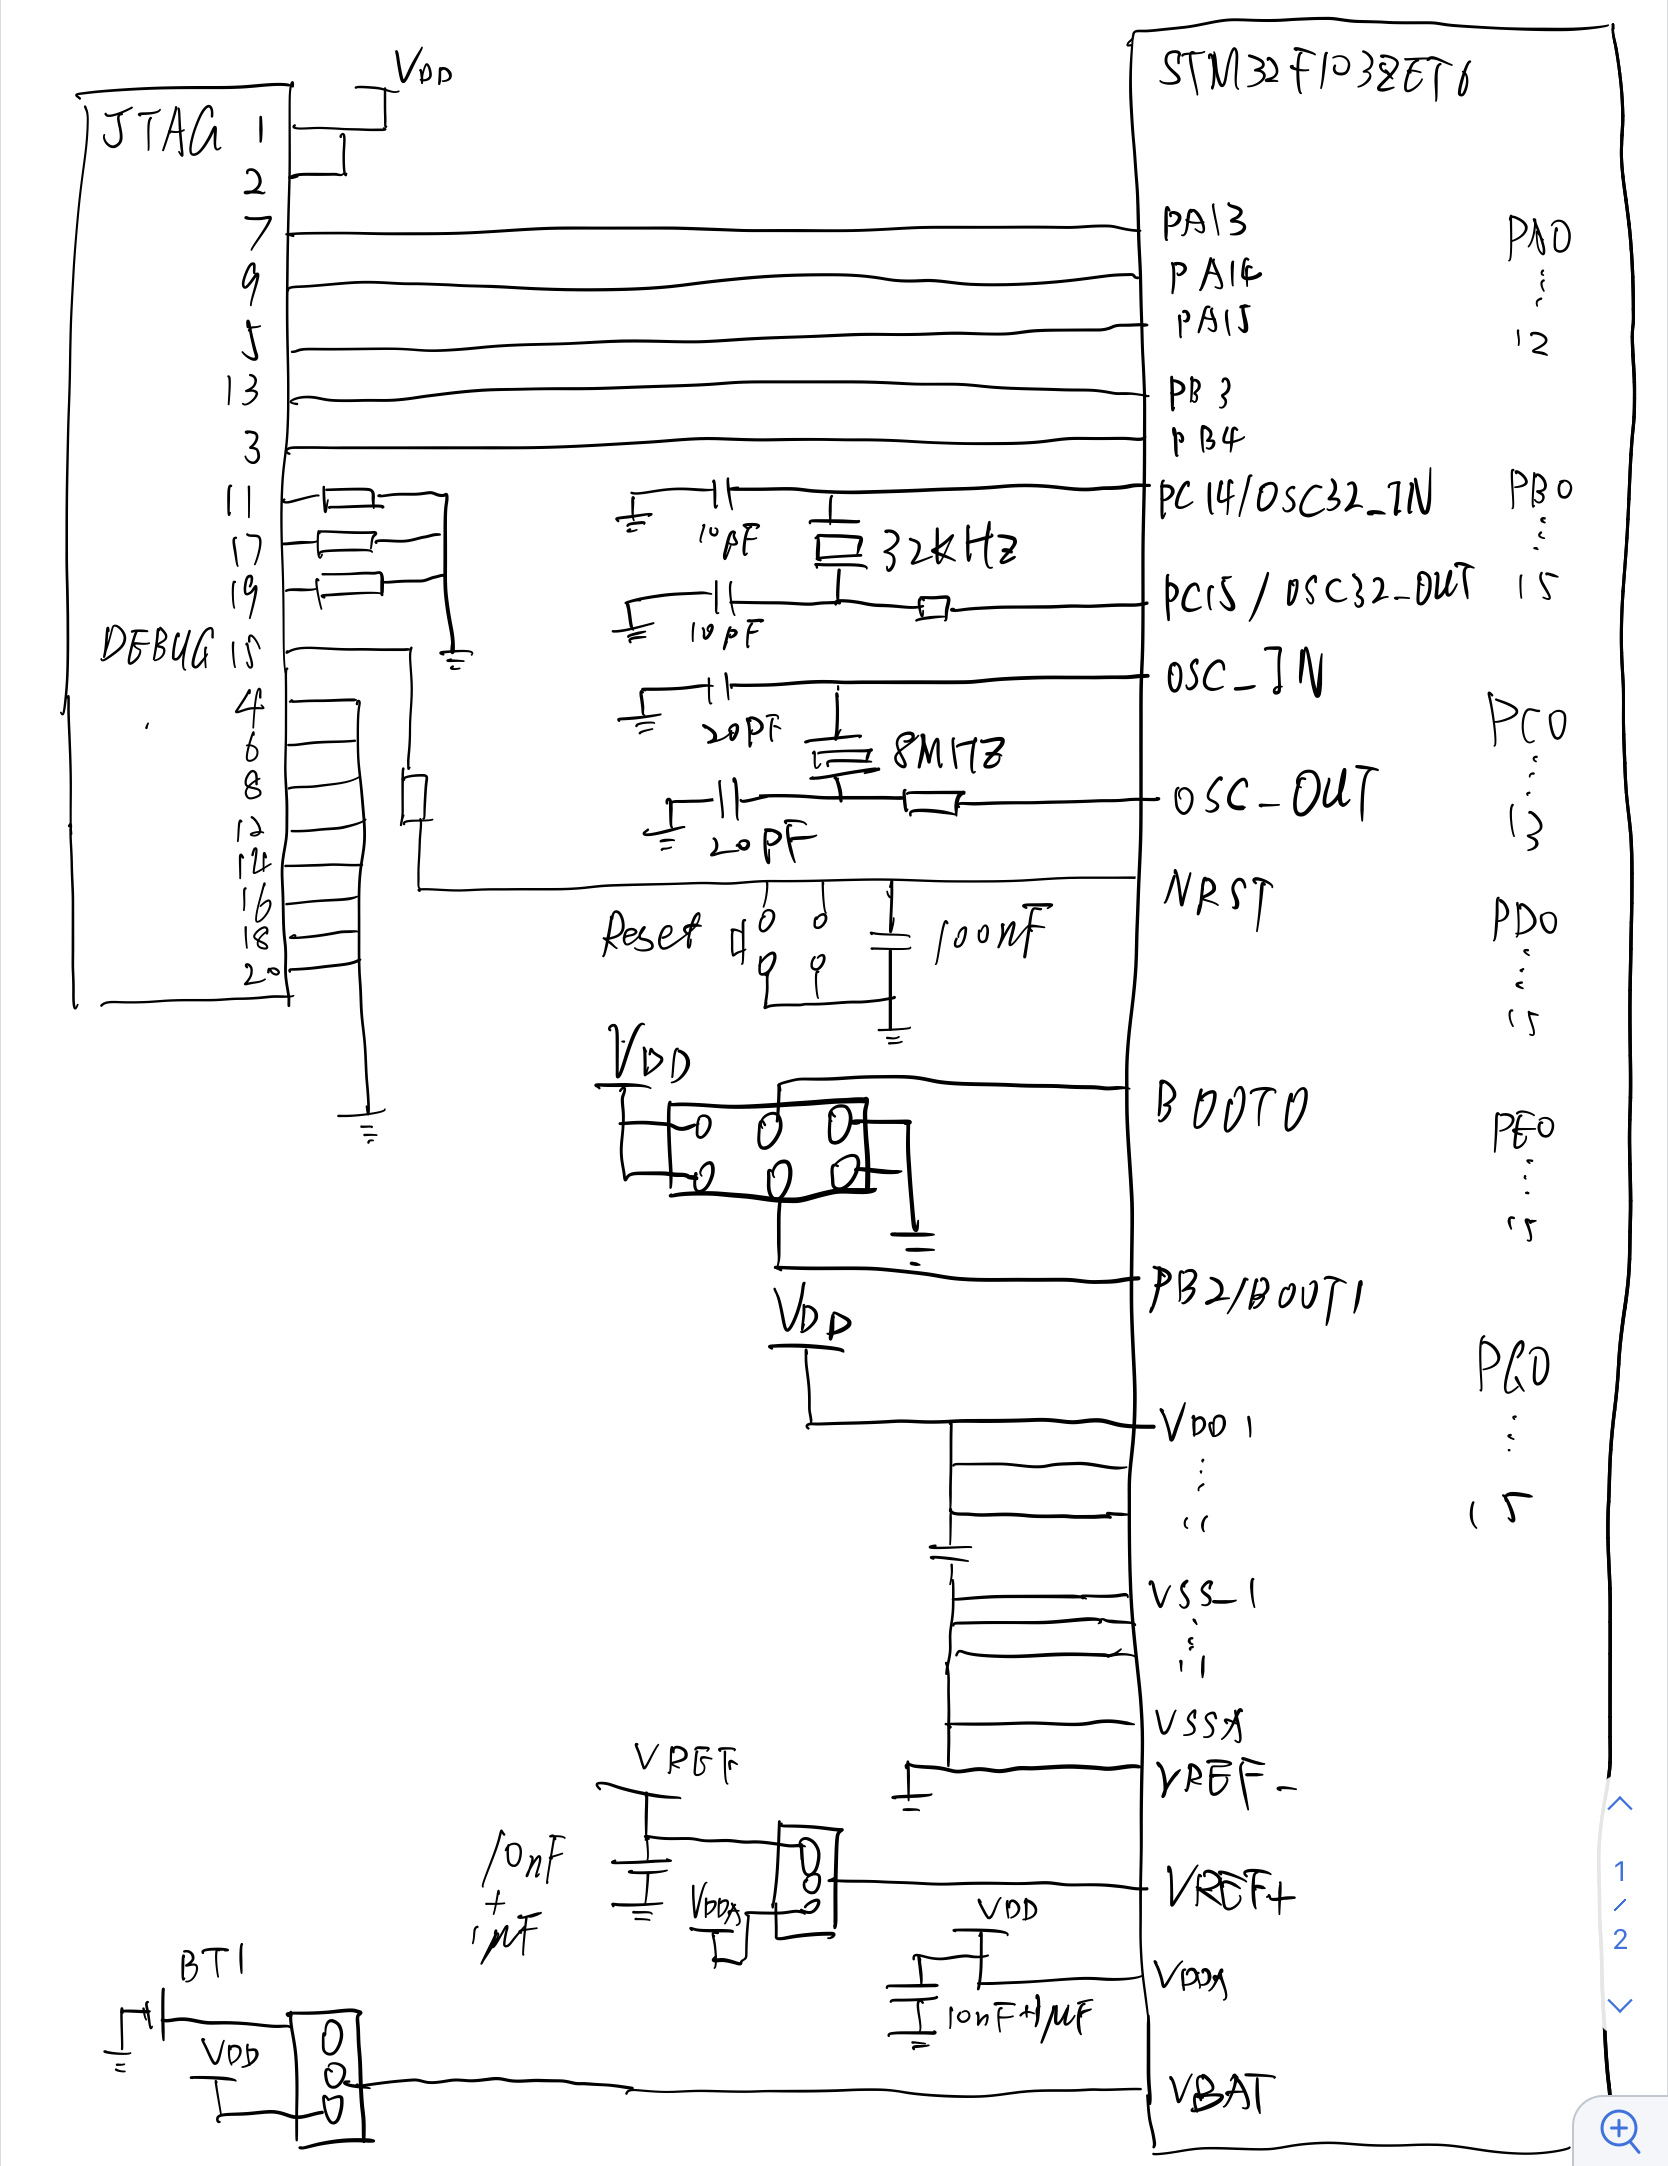
\includegraphics[scale=0.3]{1.jpeg}
    \end{figure}
    \\[4pt]\par

    \noindent\textbf{8.12}STM32F103的复位电路有何功能?常见的复位方式有哪些?\par
    微处理器上电时的电压并非突变,而是逐步上升到正常工作范围,平时供电电压不稳定时也会出现这种情况,微处理器和芯片内的程序在这段时期无法正常运行。复位电路可以给微处理器延时,使其保持在复位状态、暂不工作,防止其执行错误指令,直到电压稳定为止都保持在处理器的初始状态。\par
    复位方式:手动按键复位、WWDG看门狗、软件复位、低功耗复位、IWDG看门狗。
    \\[4pt]\par

    \noindent\textbf{8.16}参照STM32的时钟树,请做以下思考,并解释1)设计成这种形式的主要目的和理由为何?2)从左至右,相关时钟依次可分为大致哪几种?3)时钟输出的使能有何意义。\par
    1)用同一个时钟源分裂出不同频率的时间信号,这样可以保证不同频率信号之间的同步。\par
    2)输入时钟、系统时钟、从系统时钟分频得到的时钟。\par
    3)只有设定好参数并使能时钟才能让时钟按照预设的参数正常工作。
    \\[4pt]\par

    \noindent\textbf{8.27}GPIO的复用功能重映射有何意义?如何实现的,举一个例子说明。\par
    意义:可以将某外设的复用功能从默认的引脚转到备用的引脚上,方便外设的分时复用、优化引脚布局等等。\par
    例子:PB10主功能为PB10,默认复用功能是USART3的发送端$Tx$、$I^{2}C2$的时钟端SCL,重定义功能是TIM2\_CH3。上电复位后PB10为默认普通输出,如要使用默认复用功能的$I^{2}C2$,则要配置PB10为推挽输出模式,使能$I^{2}C2$并保持USART3禁止状态。若要使用PB10的重定义复用功能TIM2\_CH3,则需编程对TIM2进行重映射,然后再按复用功能方式配置。
    \\[4pt]\par

    \noindent\textbf{8.31}简述通用定时器的输入捕获过程。\par
    输入时通过检测TIMx\_CHx通道的上下沿信号,将当前TIMx\_CNT的值存到TIMx\_CCRx里进行捕获和比较,完成一次捕获。
    \\[4pt]\par

    \noindent\textbf{8.32}*参照书中例子,采用TIM2通道2进行频率测量,利用库函数实现其设置。\par
    代码如下。

    \begin{lstlisting}[language=C]
        TIM_ICInitStructure.TIM_ICMode=TIM_ICMode_ICAP; 
        TIM_ICInitStructure.TIM_Channel=TIM_Channel_2;
        TIM_ICInitStructure.TIM_ICPolarity=TIM_ICPolarity_Rising;
        TIM_ICInitStructure.TIM_ICSelection=TIM_ICSelection_DirectTI;
        TIM_ICInitStructure.TIM_ICPrescaler=TIM_ICPSC_DIV1; 
        TIM_ICInitStructure.TIM_ICFilter=0x0;
        TIM_ICInit(TIM2,&TIM_ICInitStructure);
        TIM_SelectInputTrigger(TIM2,TIM_TS_TI1FP1);
        TIM_SelectSlaveMode(TIM2,TIM_SlaveMode_Reset); 
        TIM_SelectMasterSlaveMode(TIM2,TIM_MasterSlaveMode_Enable);
    \end{lstlisting}

    \noindent\textbf{8.34}简述通用定时器的比较输出过程。\par
    定时器的CNT跳变到和捕获器CCR的值相等时,相应输出引脚可以根据编程预设选择置位、复位、翻转、不变四种输出之一,同时设置将状态寄存器SR。如果对应的中断屏蔽位置位,中断使能,则产生中断。如DMA请求位置位,则产生DMA请求。
    \\[4pt]\par

    \noindent\textbf{8.36}*参照书中例子,设计一个红绿灯系统,要求:红灯亮5秒钟,熄灭,切换绿灯亮5秒钟,熄灭,循环往复。给出硬件原理图,并编写代码实现。\par
    \begin{lstlisting}[language=C]
        //LED1和LED2的负极分别接到PA8和PA9上,正极在串限流电阻后接VCC
        //头文件略
        void gpioInit(void){
            GPIO_InitTypeDef  GPIO_InitStrxuct;
            RCC_APB2PeriphClockCmd(RCC_APB2Periph_GPIOA, ENABLE);
            GPIO_InitStruct.GPIO_Mode = GPIO_Mode_Out_PP;
            GPIO_InitStruct.GPIO_Speed = GPIO_Speed_2MHz;
            GPIO_InitStruct.GPIO_Pin = GPIO_Pin_8;
            GPIO_Init(GPIOA,&GPIO_InitStruct);
            GPIO_ResetBits(GPIOA, GPIO_Pin_8);
            GPIO_InitStruct.GPIO_Pin = GPIO_Pin_9;
            GPIO_Init(GPIOA,&GPIO_InitStruct);
            GPIO_ResetBits(GPIOA, GPIO_Pin_9);
        }
        int main(void)
        {
            delay_init();
            while(1) {
    
                GPIO_SetBits(GPIOA, GPIO_Pin_8);//LED1 OFF
                GPIO_ResetBits(GPIOA, GPIO_Pin_9);//LED2 ON
                delay_ms(5000);
                GPIO_SetBits(GPIOA, GPIO_Pin_9);//LED2 OFF
                GPIO_ResetBits(GPIOA, GPIO_Pin_8);//LED1 ON
                delay_ms(5000);
            }
        }

    \end{lstlisting}

    \noindent\textbf{Hint:}\quad View this HW github repositry at:\par
    \quad \url{https://github.com/cabasky/2021F-Embedded_System_HW}
    \\[4pt]\par
\end{document}